%dvipdfmx interim_sample.dvi

\documentclass[a4j, twocolumn]{jsarticle}
\usepackage{dendentitle}
\usepackage{amsmath, amssymb, bm, setspace}
\usepackage{cite}
\usepackage{subfigure}
%\bibliographystyle{junsrt}

\newcommand{\argmax}{\mathop{\rm arg~max}\limits}

\def\vector#1{\mbox{\boldmath $#1$}}
\renewcommand{\figurename}{fig.}
\renewcommand{\refname}{References}

% set margines
\setlength{\topmargin}{-15mm}
\setlength{\textheight}{252mm}
\setlength{\textwidth}{165mm}
\setlength{\oddsidemargin}{0mm}
\setlength{\evensidemargin}{0mm}

\setstretch{1.0}


\usepackage[dvipdfmx]{graphicx}
%\usepackage{apalike}
%\bibliographystyle{apalike}

\title{スピン波を用いた物理リザバーコンピューティングによる波形分類\\Waveform classification using spin-wave-based physical reservoir computing}
\author{廣瀬研究室 修士過程1年 37-196445 市村 剛大}
\date{2019年10月15日}

\begin{document}

\makedendentitle{輪講資料}{指導教員 廣瀬 明}

\section*{Abstract}


\section{はじめに}
近年、ディープラーニングをはじめとしたパターン認識の実用化が活発化しているが、その一方でその膨大な消費エネルギーが問題となっている。より省電力でパターン認識を行えるような需要が増しており、その期待に応えるものとして物理リザバーコンピューティング(Physical Reservoir Computing:PRC)というニューロ的な計算手法が注目されている。

リザバーコンピューティング(RC)はリカレントニューラルネットワーク(RNN)の一種であり、時系列データを直接扱うことができ、また学習コストが低く、早い学習を実現するニューラルネットワークである。また、その性質から物理的実装が容易であり、様々な方法で実装が試みられている。これらの試みは物理リザバーコンピューティングと呼ばれている。一般に、非線形性、短時間記憶性、の二つの性質を兼ね備える物理的ダイナミクスは、物理リザバーコンピューティングに応用することができる可能性があり、レーザー光\cite{opt}、メモリスタ、スピン波\cite{spin_reservoir}といった実用化を念頭に置いたものから、タコ足ソフトロボット\cite{Nakajima2015SciReo:_infor_proce_via_physi_soft_body}、バケツの水\cite{Fernando2003AL:_patter_recog_in_a_bucke}といったユニークなものまで様々な物理的ダイナミクスを利用して物理リザバーコンピューティングが行われている。

\begin{figure}
\centering
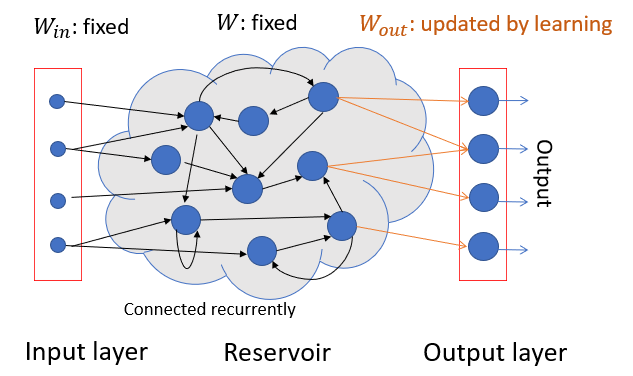
\includegraphics[width=1\hsize]{./figures/esn}\\
\caption{Concept of Echo State Network(ESN).}
\label{fig:esn}
\end{figure}

\section{背景}
\subsection{リザバーコンピューティング}
リカレントニューラルネットワーク(RNN)は再帰的な構造を持つニューラルネットワークであり、その構造から、パーセプトロンやディープラーニングで用いられるような層状のニューラルネットワークとは異なり、時系列データをそのまま処理することができる。しかしRNNは層状ニューラルネットワークに比べニューロン間の結合が多くなり、それらの間の結合荷重を勾配法などによって全て更新しようとするとニューロン数に対して莫大な計算量が必要になってしまうという問題があった。そこで2001年にJeagerによって提案されたRNNがEcho State Network(ESN)\cite{esn}である。

ESNは図\ref{fig:esn}に示されるようなニューラルネットワークであり、通常のRNNとは異なり入力層の結合荷重$W^{in}$とリカレントな部分の結合荷重$W$はランダムな値で固定されており、読み出し部の結合荷重$W^{out}$のみを可変し、学習によって更新するというものである。ニューロンがリカレント構造をなしている部分はリザバー(Reseivoir)と呼ばれる。リザバーはため池という意味で、この部分に過去に入力された情報がたまることに由来している。
ESNにおいてリザバー内の各ニューロンの状態は以下の式のように表される。
\begin{eqnarray}
\label{eq:esn1}
	\mathbf{x}(n) = \mathbf{f}(W^{in}\mathbf{u}(n) + W\mathbf{x}(n-1)),
\end{eqnarray}
ここでnは離散時間を表しており、$\mathbf{x}$はリザバーの内部状態ベクトル、$\mathbf{u}$はリザバーの入力行列、$W$はリザバーの結合荷重行列、$W^{in}$は入力層の荷重行列である。ESNでは出力層の荷重のみが可変なので、$W$と$W^{in}$はリザバーごとに固有の、固定された行列となる。$\mathbf{f}$はニューロンの活性化関数であり、何らかの非線形関数が用いられる。$\mathbf{f}(x) = 1/(1 + \exp(-x))$(シグモイド関数)や、$\mathbf{f}(x) = \tanh(x)$がよく用いられる。$\mathbf{x}(n)$を定める式(\ref{eq:esn1})の項に$\mathbf{x}(n-1)$が入っていることが、ESNが時系列データを扱っていることを意味している。出力は次のように表される。
\begin{eqnarray}
\label{eq:esn2}
	\mathbf{y}(n) = \mathbf{f_{out}}(W^{out}\mathbf{x}(n)),
\end{eqnarray}
$\mathbf{y}(n)$はnにおける出力ベクトル、$W^{out}$は出力層の結合荷重である。また$f_{out}$は出力ニューロンの活性化関数で任意の関数であり、線形和でも十分機能することが多い。$W^{out}$は$W$や$W^{in}$と異なり学習によって変化する。具体的には、ムーア・ペンローズの擬逆行列などを用いて求めることができる。或いはオンラインに荷重を更新したい場合や学習用データが膨大な場合は、教師出力と実際の出力の二乗誤差の和やクロスエントロピーをコスト関数とし、そのコスト関数を最小化するような方向に$W^{out}$を変化させるような方法がよく用いられ、これは勾配法と呼ばれている。

\begin{figure}
\centering
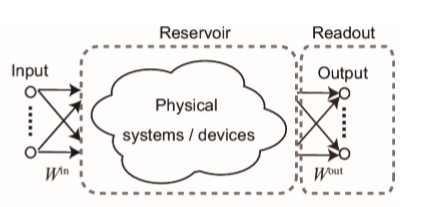
\includegraphics[width=1\hsize]{./figures/phisicalrc2}\\
\caption{Concept of Phisical Reservoir Computing(PRC)\cite{tanaka2018recent}.You can see reservoir neurons in reservoir are replaced by phisical systems/devices comparing with ESN(fig.1).}
\label{fig:prc}
\end{figure}

\subsection{物理リザバーコンピューティング}
リザバーコンピューティングにおけるリザバー内のふるまいを、物理的なダイナミクスを用いて置き換えることでリザバーコンピューティングを物理的に実装しようとする試みが近年活発に行われており、これらは物理リザバーコンピューティング(PRC、物理RC)と呼ばれている(図\ref{fig:prc})。物理RCは現行のフォンノイマン型のコンピュータを用いたパターン認識とは異なり、物理的に直接パターン認識を行っているという点で従来のものとは一線を画す、新しい視点の計算法である。リザバーコンピューティングを行う上では物理RCはフォンノイマン型のコンピュータより早く、省エネルギーでパターン認識が行える可能性があり注目されている。またリザバーのランダム性を逆手にとって、デバイスの製造に精度が求められない、「作りこまないデバイス」を設計することも可能である\cite{ahirose2019J_IEICE:_prosp_for_reser_compu}。
一般に、非線形性、短時間記憶性、の二つの性質を兼ね備える物理的ダイナミクスは、物理リザバーコンピューティングに応用することができる可能性がある。


物理リザバーコンピューティングに非常に様々な物理的ダイナミクスが利用できる例として、図\ref{fig:liquidbrain}のようなバケツの中の水面波を利用したもの\cite{Fernando2003AL:_patter_recog_in_a_bucke}、図\ref{fig:soft}のような水中におけるタコ足ソフトロボットの動きを利用したもの\cite{Nakajima2015SciReo:_infor_proce_via_physi_soft_body}などが挙げられる。

\subsection{スピン波リザバーコンピューティング}
波動利用のリザバーとして、スピン波を利用するリザバーコンピュータの概念とその構成、基礎的な検証も報告されている\cite{Nakane2018IEEEAccess:_Reser_Compu_with_spin_waves_Excit_in_a_Garne_film,Nakane2018ICM:_demon_of_spin_wave_based_reser_compu_for_next_gener_machi_learn_devic}。そこでは、方形波として時間的に変化するベースバンド信号を入力信号とした。そしてその方形波の継続時間を推定するタスクを設定し、これに成功した。このスピン波リザバーコンピューテイングデバイスは、波動現象を利用している。すなわち、ヒステリシス、非線形性、空間的な非対称性などを利用するとともに、波動としての分散特性も利用できる。この場合、ヒステリシスは入力信号と入力端との相互作用が、入力端の状態に依存していることを意味するとともに、伝搬もヒステリシスを有している。非線形性は、波の性質が波動の振幅に依存していること、たとえば干渉の際に波動が単なる重ね合わせではない値をとり、また高次周波数成分を発生することにつながる。また非対称性は、2次元または3次元的に波動が伝搬する際に異方性があることを指す。そこでは、スピン波の時空間的な特性が直接にリザバーの機能の豊かさを規定する。
先行研究\cite{Nakane2018IEEEAccess:_Reser_Compu_with_spin_waves_Excit_in_a_Garne_film}では基本的な構成、検証にとどまっており、また計算方法は、得られた振幅の値を時間方向に展開してから計算を行うため、2次元波であることによる空間的な情報を十分に利用していない。そこで

\begin{figure}
\centering
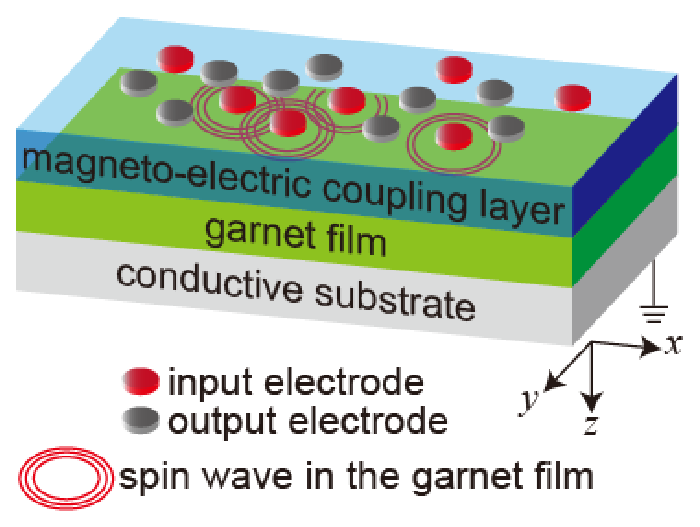
\includegraphics[width=0.9\hsize]{./figures/deviceStructure.eps} 
\caption{Basic structure of spin-wave reservoir computing device.(Figure reproduced under permission from IEEE.)}
\label{fig:basicstrct}
\end{figure}

\begin{figure}
\centering
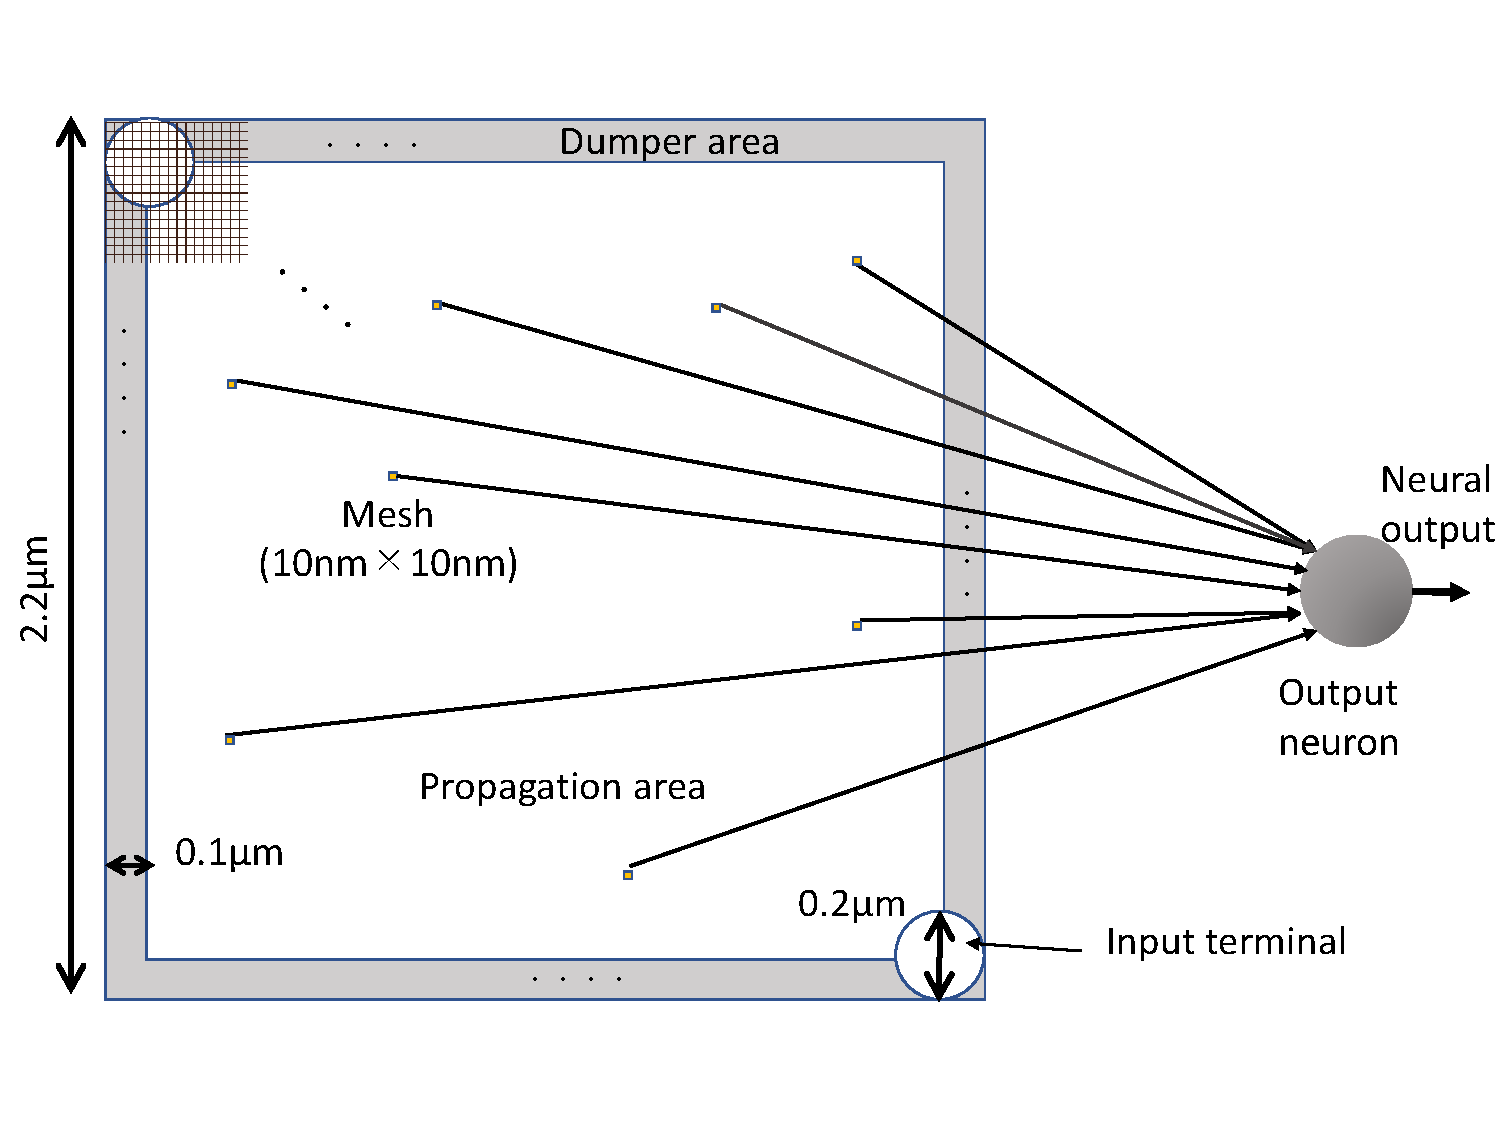
\includegraphics[width=0.9\hsize]{./figures/selected_neuron_structure.pdf} 
\caption{Structure of the network.}
\label{fig:sond}
\end{figure}

\section{スピン波リザバーの構成とタスク}%%%%%%%%%%%%%%%%%%%%%%%%%%%%%%%%%%%%%%%%%%%%%%%%%%%%%%%%%%%%%%%%%%%%%%%%%%%%%%
%\section{Construction of the spin-wave reservoir}
\label{sec:constandtask}

\subsection{物理的な構成}
\label{subsec:const}

図\ref{fig:basicstrct}は素子の基本構造の概念図である。物理的な詳細は、先行研究と同様のものを用いた\cite{Nakane2018IEEEAccess:_Reser_Compu_with_spin_waves_Excit_in_a_Garne_film,Nakane2018ICM:_demon_of_spin_wave_based_reser_compu_for_next_gener_machi_learn_devic}。簡単には、入力電極に電圧を加えることにより、ME結合層で生じるME結合によって、ガーネットフィルムのスピンに波動を誘起することができる。その波動はフィルム内を伝搬する。その際、波動は異方性を伴いながら伝搬したり、非線形性を伴いながら干渉したりする。また入力電極やフィルムでの波動伝搬は、新たな信号に対しヒステリシスを持つ。このような特性から、スピン波自体が時系列入力信号を複雑な時系列信号に変換する。これがスピン波リザバーの効果的な動作である。このような複雑なスピン波動を入力と同様に出力電極でME結合によってピックアップし、出力信号を得る。
%Fig.~\ref{fig:structure} is a conceptual illustration showing the basic construction of the garnet-film spin reservoir. Physical details are given in literature~\cite{Nakane2018IEEEAccess:_Reser_Compu_with_spin_waves_Excit_in_a_Garne_film,Nakane2018ICM:_demon_of_spin_wave_based_reser_compu_for_next_gener_machi_learn_devic}. The dynamics is explained simply as follows. Input voltage at terminals triggers spin waves in the garnet film. The spin wave propagates, interferes and bounces at the edges with nonlinearity, anisotropy and hysteresis. These phenomena transform the time-sequential input signals into complicated spatiotemporal signals, which works effectively as a reservoir. 

図\ref{fig:sond}に本論文での解析のためのフィルムの大きさと2つの入力電極を示す。ここで、2つの入力端子を設置するのはスピン波の非線形な干渉を利用するためである。干渉を利用する場合としない場合の性能の評価は先行研究でなされている\cite{Nakane2018IEEEAccess:_Reser_Compu_with_spin_waves_Excit_in_a_Garne_film,Nakane2018ICM:_demon_of_spin_wave_based_reser_compu_for_next_gener_machi_learn_devic}。

\subsection{正弦波/矩形波分類タスク}
\label{subsec:task}

タスクには正弦波/矩形波の分類を採用する。リザバーコンピューティングを含むRNNの特徴として時系列データをそのまま扱うことができるという特徴があり、時系列処理が正弦波/矩形波分類はこの特徴を生かせるタスクである。2端子にそれぞれ、周波数$f=2.5~\rm{GHz}$ (周期$T=0.4$~ns)の正弦波、矩形波を入力する。ただし、今回は理想的な矩形波の代わりに式(\ref{eq:term4})のように第4項までフーリエ級数展開した矩形波を用いた。
\begin{eqnarray}
	f_{square}(t) = \mathrm{cos}\biggl( \frac{2{\pi}t}{T}\biggr)-\frac{1}{3}\mathrm{cos}\biggl(\frac{3\times2{\pi}t}{T}\biggr) \nonumber \\
	\quad\quad\quad  +\frac{1}{5}\mathrm{cos}\biggl(\frac{5\times2{\pi}t}{T}\biggr)-\frac{1}{7}\mathrm{cos} \biggl(\frac{7\times2{\pi}t}{T}\biggr)
\label{eq:term4}
\end{eqnarray}
これは、現実的に入力される電圧は理想的な矩形波よりも立ち上がりがなまったものと考えられるからである。2端子には同じ波形を入力し、正弦波を入力したときは"0"が、矩形波が入力されたときは"1"が出力ニューロンから出力されるよう学習を行う。縦軸の入力信号に対応して変調される物理量は、magnetocrystalline anisotropy constant $K_{u}$であり、電圧入力によってこれを等価的に変化させる。なお、以下のスピン波解シミュレーション析にはシミュレータMuMax3を用いた\cite{Vansteenkiste2014AIP:_the_desig_and_verif_of_MuMax}。$x$--$y$平面内の空間メッシュは10~nm四方、時間ステップは0.01~nsとした。
%Fig.~\ref{fig:film} shows the dimension of the film chip as well as the sizes and positions of the input electrodes A and B. We assume a task of exclusive or (XOR) in this paper. We prepare "0""0", "0""1", "1""0" and "1""1" inputs, where the voltage waveforms are similar to those in our previous work \cite{Nakane2018IEEEAccess:_Reser_Compu_with_spin_waves_Excit_in_a_Garne_film} as shown in Fig.~\ref{fig:inputSignals}. The physical property to be modulated is the magnetocrystalline uniaxial anisotropy constant $K_{u}$ in the film. In the following simulation experiments, we used MuMax3 simulator \cite{Vansteenkiste2014AIP:_the_desig_and_verif_of_MuMax}. The spatial mesh size is 1~$\mu$m square, and the time step is 0.01~ns. 

\subsection{学習方法}
\label{subsec:learning}

図\ref{fig:sond}にリザバーニューラルネットワークの全体の構成も示す。リザバー出力信号は、出力ニューロンの入力信号でもある。ここでは出力電極の大きさをシミュレータのメッシュ一つ分と仮定した。これらのリザバー出力(信号$\bm{x}$)を前処理の後、出力ニューロンに、シナプス結合(荷重$\bm{w}$)を介して供給する。ニューロンには$f ( u ) = (1/(1+\exp(-u)))$型の非線形活性化関数を仮定し、出力信号を出力する。可変閾値も準備している。
%Fig.~\ref{fig:network} shows the total construction of the reservoir neural network. The output of the reservoir is fed to a neuron. In this paper, we prepare about 220$\times$220 very small and dense output electrodes virtually pixel by pixel of the numerical mesh size. The reservoir output $\bm{x}$ are simply preprocessed and fed to the neuron through weights $\bm{w}$. The neuron has an activation function with nonlinearity of $f ( u ) = ( 1 / ( 1 + \exp ( - u ) ) )$ to generate a neural output. The neuron has a bias term as well. 

本解析では、場所$\bm{r}$でのニューロン出力の包絡線振幅を観測する。場所$\bm{r}$、フレーム$n$でのリザバー出力ベクトル$x(\bm{r},n)$は、スピン波の振幅の時系列データ$s_{x}(\bm{r},n)$から次のように求められる。
%In this experiment, we observe the amplitude at position $\bm{r}$ averaged in time $t$=$t_{\rm e}$~--~$T$ with a rectification and low-pass filtering (LPF) preprocess. That is, 
%
\begin{eqnarray}
\hspace*{-1em} 
x(\bm{r}, n)
=
{\rm Amp} (s_{x}(\bm{r}, n)-s_{x}^{\rm offset}(\bm{r}))
\label{eq:yn} 
\end{eqnarray}
ただし${\rm Amp}(\cdot)$はスピン波の振幅を表し、今回のシミュレーションではヒルベルト変換したものの絶対値を用いた。現実的にはアナログ的にダイオードによる整流を行う。学習用データ全体に対して出力値$y ( n )$と正弦波/矩形波に対応する教師信号$\hat{y} ( n )$=1あるいは0によって、ミニバッチ学習を行う。ミニバッチ学習は比較的多くのデータを扱う学習を行う際に用いられる学習方法であり、次のような手順で学習が行われる。
%where ${\rm Amp} ( \cdot )$ denotes amplitude extraction and $w_{0}$ is the neuron bias to be appended to $\bm{w}$. This process is realized by a diode and a LPF very easily in reality. In (\ref{eq:yn}),  $n$ is an index for time frame. In the present task, every time-sequential signal is processed within a time frame almost independently though there exists time-dependent processing within a time frame. We apply a supervised learning employing the gradient descent method to minimize the difference of neural output $y ( n )$ and the XOR teacher signal $\hat{y} ( n )$=1 or 0 in every time frame $n$ as 
%
まず、学習に用いる$N$個のデータセットを$N/N_{\rm mini}$個の、$N_{\rm mini}$個のデータからなるデータセットに分ける。次に、あるミニバッチのデータ全てに対して次式のように荷重$\bm w$を$\bm w_{new}$に更新する。
\begin{eqnarray}
\Delta \bm{w} &=& - \frac{\eta}{N_{\rm mini}} \sum^{N_{\rm mini}} ( y ( n ) - \hat{y} ( n ) ) f'( \bm{w} \cdot {\bm{x}} ) \bm{x}
\label{eq:Deltabmw1}
\end{eqnarray}
\begin{eqnarray}
\bm{w}_{\rm new} = \bm{w} + \Delta \bm{w}
\label{eq:Deltabmw2}
\end{eqnarray}
ここで$\eta$は学習係数である。$f'(\cdot)$は非活性関数$f ( u ) = (1/(1+\exp(-u)))$を$u$で微分したものである。なお、$\bm{w}$,$\bm{x}$はバイアス成分も含み表記している。
%where $\varepsilon$ is a small positive real number. 
同様の操作を$N/N_{\rm mini}$個のデータ全てに対して行う。学習データをすべて用い、一周学習することを1エポックと数える。


\begin{figure}
\centering
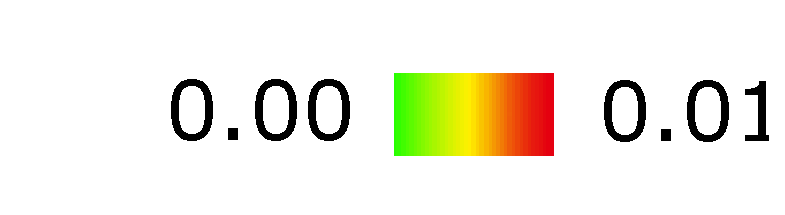
\includegraphics[width=0.4\hsize]{./figures/colorbar_001.eps} \\
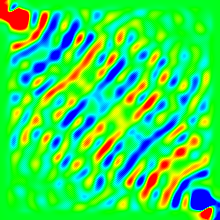
\includegraphics[width=0.4\hsize]{./figures/capture/sin/sinsqr128_32i_l_dif_5760} \ 
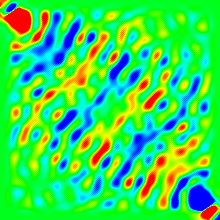
\includegraphics[width=0.4\hsize]{./figures/capture/sin/sinsqr128_32i_l_dif_5761} \\
%frame 4480 \hspace*{0.2\hsize} frame 4481  \vspace{5pt}\\
%0/40 T \hspace*{0.3\hsize} 1/40 T  \vspace{5pt}\\
0.000\ $T$ \hspace*{0.25\hsize} 0.025\ $T$  \vspace{5pt}\\
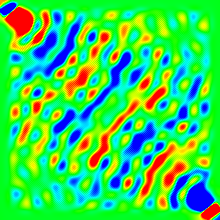
\includegraphics[width=0.4\hsize]{./figures/capture/sin/sinsqr128_32i_l_dif_5762} \ 
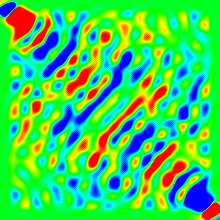
\includegraphics[width=0.4\hsize]{./figures/capture/sin/sinsqr128_32i_l_dif_5763} \\
%frame 4482 \hspace*{0.2\hsize} frame 4483  \vspace{5pt}\\
%2/40 T \hspace*{0.3\hsize} 3/40 T  \vspace{5pt}\\
0.050\ $T$ \hspace*{0.25\hsize} 0.075\ $T$  \vspace{5pt}\\
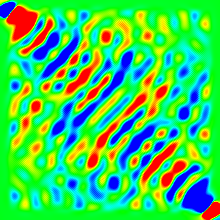
\includegraphics[width=0.4\hsize]{./figures/capture/sin/sinsqr128_32i_l_dif_5764} \ 
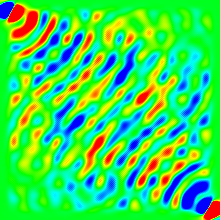
\includegraphics[width=0.4\hsize]{./figures/capture/sin/sinsqr128_32i_l_dif_5766} \\
%frame 4484 \hspace*{0.2\hsize} frame 4485  \vspace{5pt}\\
%4/40 T \hspace*{0.3\hsize} 5/40 T  \vspace{5pt}\\
0.100\ $T$ \hspace*{0.25\hsize} 0.125\ $T$  \vspace{5pt}\\
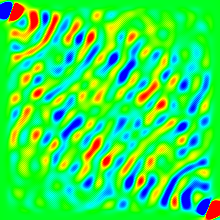
\includegraphics[width=0.4\hsize]{./figures/capture/sin/sinsqr128_32i_l_dif_5767} \ 
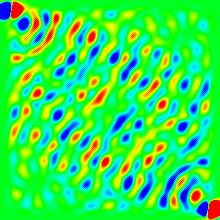
\includegraphics[width=0.4\hsize]{./figures/capture/sin/sinsqr128_32i_l_dif_5768} \\
%frame 4486 \hspace*{0.2\hsize} frame 4487  \vspace{5pt}\\
%6/40 T \hspace*{0.3\hsize} 7/40 T  \vspace{5pt}\\
0.150\ $T$ \hspace*{0.25\hsize} 0.175\ $T$  \vspace{5pt}\\
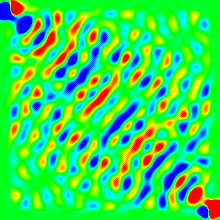
\includegraphics[width=0.4\hsize]{./figures/capture/sin/sinsqr128_32i_l_dif_5769} \ 
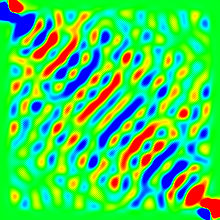
\includegraphics[width=0.4\hsize]{./figures/capture/sin/sinsqr128_32i_l_dif_5770} \\
%frame 4488 \hspace*{0.2\hsize} frame 4489  \vspace{5pt}\\
%8/40 T \hspace*{0.3\hsize} 9/40 T  \vspace{5pt}\\
0.200\ $T$ \hspace*{0.25\hsize} 0.225\ $T$  \vspace{5pt}\\
\caption{
正弦波を入力した場合のスピン波の様子($s_{x}$成分)。($T$=0.4ns)
%Spin-wave propagation when we feed input electrodes A and B with “0” and “1”, respectively.
}
\label{fig:waves1xsin}
\end{figure}

\begin{figure}
\centering
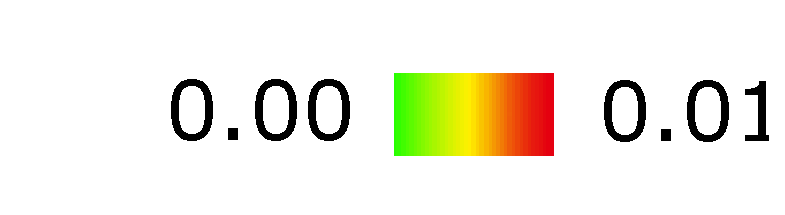
\includegraphics[width=0.4\hsize]{./figures/colorbar_001.eps} \\
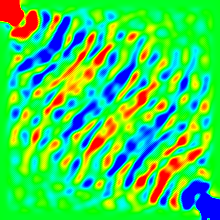
\includegraphics[width=0.4\hsize]{./figures/capture/sqr/sinsqr128_32i_l_dif_7060} \ 
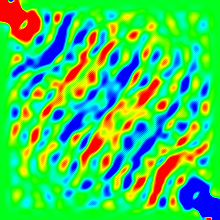
\includegraphics[width=0.4\hsize]{./figures/capture/sqr/sinsqr128_32i_l_dif_7061} \\
%frame 5780 \hspace*{0.2\hsize} frame 5781  \vspace{5pt}\\
0.000\ $T$ \hspace*{0.25\hsize} 0.025\ $T$  \vspace{5pt}\\
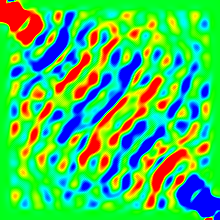
\includegraphics[width=0.4\hsize]{./figures/capture/sqr/sinsqr128_32i_l_dif_7062} \ 
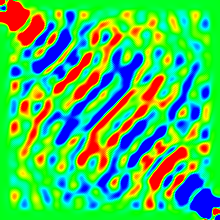
\includegraphics[width=0.4\hsize]{./figures/capture/sqr/sinsqr128_32i_l_dif_7063} \\
%frame 5782 \hspace*{0.2\hsize} frame 5783  \vspace{5pt}\\
0.050\ $T$ \hspace*{0.25\hsize} 0.075\ $T$  \vspace{5pt}\\
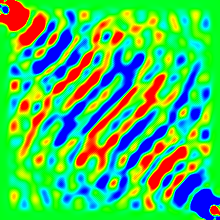
\includegraphics[width=0.4\hsize]{./figures/capture/sqr/sinsqr128_32i_l_dif_7064} \ 
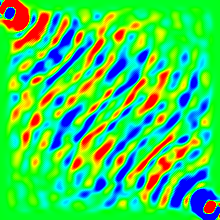
\includegraphics[width=0.4\hsize]{./figures/capture/sqr/sinsqr128_32i_l_dif_7066} \\
%frame 5784 \hspace*{0.2\hsize} frame 5785  \vspace{5pt}\\
0.100\ $T$ \hspace*{0.25\hsize} 0.125\ $T$  \vspace{5pt}\\
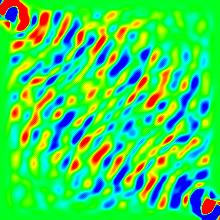
\includegraphics[width=0.4\hsize]{./figures/capture/sqr/sinsqr128_32i_l_dif_7067} \ 
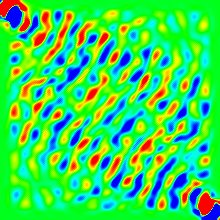
\includegraphics[width=0.4\hsize]{./figures/capture/sqr/sinsqr128_32i_l_dif_7068} \\
%frame 5786 \hspace*{0.2\hsize} frame 5787  \vspace{5pt}\\
0.150\ $T$ \hspace*{0.25\hsize} 0.175\ $T$  \vspace{5pt}\\
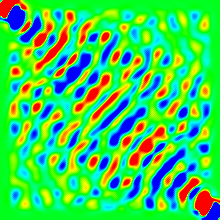
\includegraphics[width=0.4\hsize]{./figures/capture/sqr/sinsqr128_32i_l_dif_7069} \ 
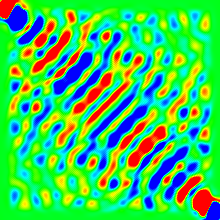
\includegraphics[width=0.4\hsize]{./figures/capture/sqr/sinsqr128_32i_l_dif_7070} \\
%frame 5788 \hspace*{0.2\hsize} frame 5789  \vspace{5pt}\\
0.200\ $T$ \hspace*{0.25\hsize} 0.225\ $T$  \vspace{5pt}\\
\caption{
第4項までフーリエ展開した矩形波を入力した場合のスピン波の様子($s_{x}$成分)。($T$=0.4ns)
%Spin-wave propagation when we feed both input electrodes A and B with “1”.
}
\label{fig:waves4xsqr}
\end{figure}

\begin{figure}
\centering
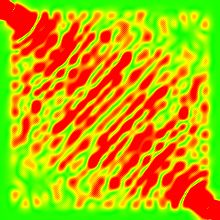
\includegraphics[width=0.5\hsize]{./figures/capture/sin/32i_l_hil_5760} \\
(a)\\
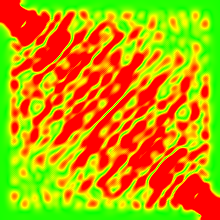
\includegraphics[width=0.5\hsize]{./figures/capture/sqr/32i_l_hil_7060} \\
(b)\\ 
\caption{(a)正弦波(b)矩形波を入力したときの振幅}
\label{fig:hil}
\end{figure}

\section{正弦波矩形波分類タスクの実験結果}%%%%%%%%%%%%%%%%%%%%%%%%%%%%%%%%%%%%%%%%%%%%%%%%%%%%%%%%%%%%%%%%%%%%%%%%%%%%%%%%
\label{sec:result}

\subsection{スピン波伝搬の様子}
\label{subsec:spinwave}

図\ref{fig:waves1xsin}は正弦波、図\ref{fig:waves4xsqr}は矩形波を2端子に入力したときのスピン波の伝搬の様子である。今回用いた周波数は$f=2.5~\rm{GHz}$であり、フレーム1枚は0.01nsであるから、40フレームで入力波の1周期である。スピン波は10GHz程度の強磁性共鳴(FMR)周波数と呼ばれる基本周波数を持っており、その周波数で赤と青が入れ替わっている。入力信号正弦波を入力したときと矩形波を入力したときでスピン波の干渉の様子が異なっていることがわかる。
%Fig.~\ref{fig:waves11x} shows the waves when we feed inputs A:"1" and B:"1". Though the reverberations in $t$=7~--~9~ns seems similar to those in Fig.~\ref{fig:waves10x}, precise comparison elucidates its difference. At $t$=9~ns, the electrode voltage arises, resulting in new waves that reflect reverberations with the hysteresis. The waves are also similar, but different from previous ones in Fig.~\ref{fig:waves11x}. 
図\ref{fig:hil}は図\ref{fig:waves1xsin}、図\ref{fig:waves4xsqr}のようなスピン波の振幅をあるフレームについて式(\ref{eq:yn})のように前処理をして求めた信号であり、またこれは出力ニューロンの入力$\bm{x}$に使用される値である。

\subsection{有用情報の分布}
\label{subsec:info}

まずガーネット薄膜上の有用情報分布を調べるために、すべてのメッシュに仮想的に出力電極が配置されているとして学習を行った。

\begin{figure}
\centering
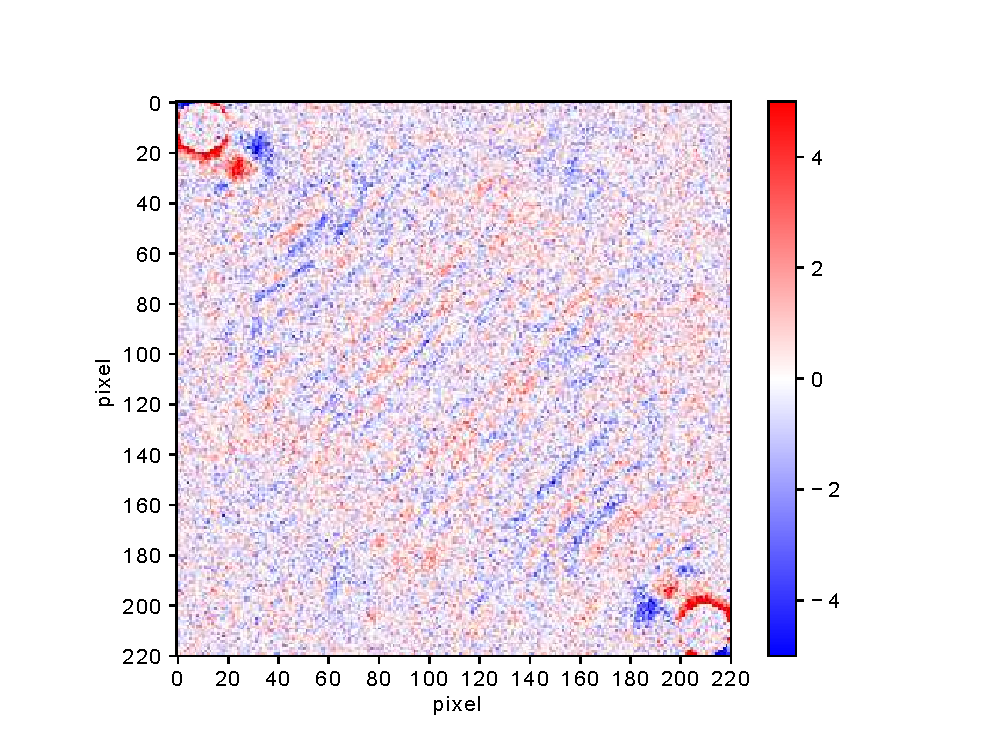
\includegraphics[width=1\hsize]{./figures/meanweightsinsqr128_32i_l_hilsinsqr128_32i_t_hil_timesequence_epoch300_batchsize32_mask10_eta30_transition0} 
\caption{荷重分布(300エポックのとき)}
\label{fig:weightsinsqr128_32i}
\end{figure}

図\ref{fig:weightsinsqr128_32i}は学習後の荷重分布である。赤い部分は正、青い部分は負の荷重であり、その色が濃いほどその絶対値が大きいことを表している。同じ色の部分が集まっている場所は同様の特徴量が得られる場所と考えることができる。中央付近に縞状に荷重の絶対値が大きい部分が分布していることが分かり、またこの幅は50~nm以上であるように見て取れる。つまり出力電極の大きさとしては今回のタスクでは数十nmが適切であると考えられる。

\begin{figure}
\centering
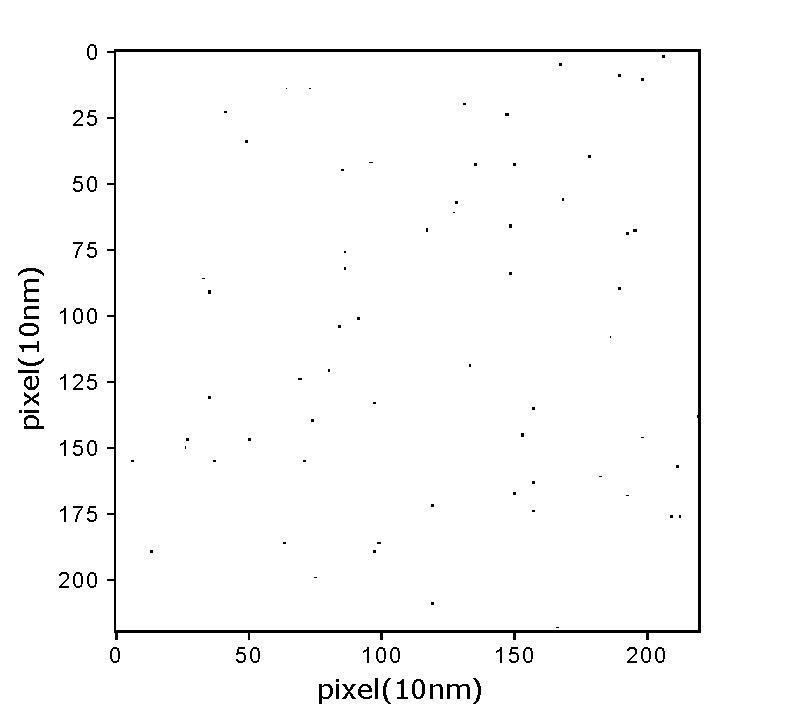
\includegraphics[width=1\hsize]{./figures/pspsinsqr128_32i_l_hilsinsqr128_32i_l2_hil_num_neuron64_ramdomselected_timesequence_epoch2000_batchsize128_mask10_eta30_transition0_loopnum9_r} 
\caption{ランダムに選択された出力電極の場所の例(出力電極数が64個の場合).}
\label{fig:random}
\end{figure}

\subsection{現実的な出力端子個数での学習}
\label{subsec:limited}

次に現実的なシミュレーションとして有限個の出力をガーネット薄膜上のランダムな位置に設定し、同様のタスクを行なった。ネットワークの概念図が図\ref{fig:sond}である。64個の電極を利用するときにランダムに選んだ電極の場所の例が図\ref{fig:random}である。入力電極上には実際には出力電極を配置することができないため、位置が選択されないようにした。

\begin{figure*}
\centering
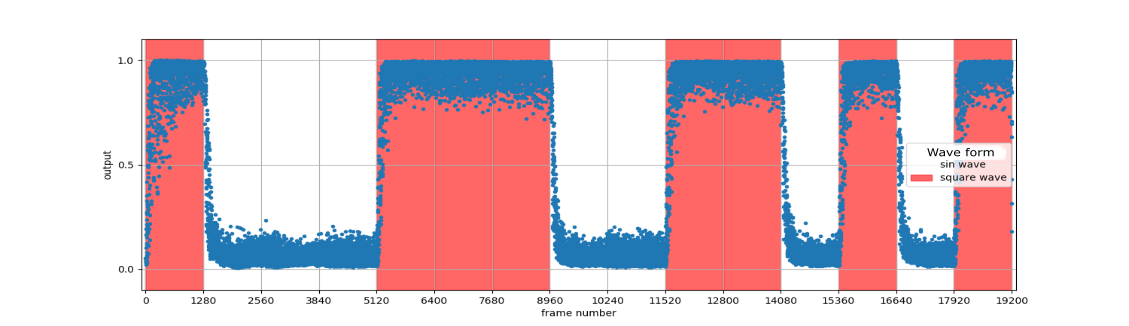
\includegraphics[width=1\hsize]{./figures/b128_e2000_eta30_nn64_r} 
\caption{Resulting neural output after learning (64~output electrodes, 2000~epoch).}
\label{fig:result64}
\end{figure*}

\begin{figure}
\centering
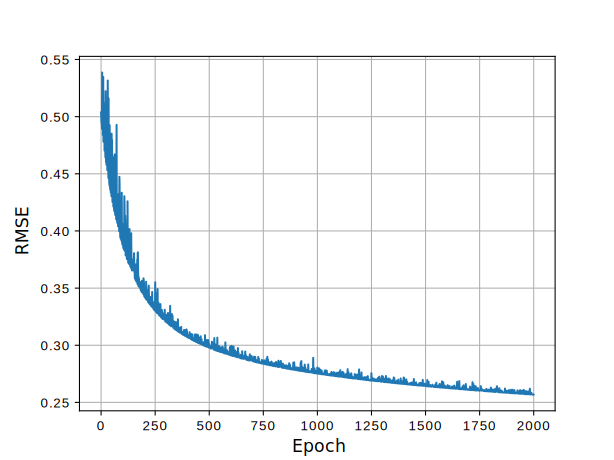
\includegraphics[width=1\hsize]{./figures/rmse_curvesinsqr128_32i_l_hilsinsqr128_32i_l2_hil_num_neuron64_ramdomselected_timesequence_epoch2000_batchsize128_mask10_eta30_transition0_loopnum9_r} 
\caption{RMSE against epoch (64~output electrodes, 2000~epoch).}
\label{fig:lc64}
\end{figure}

\begin{figure}
\centering
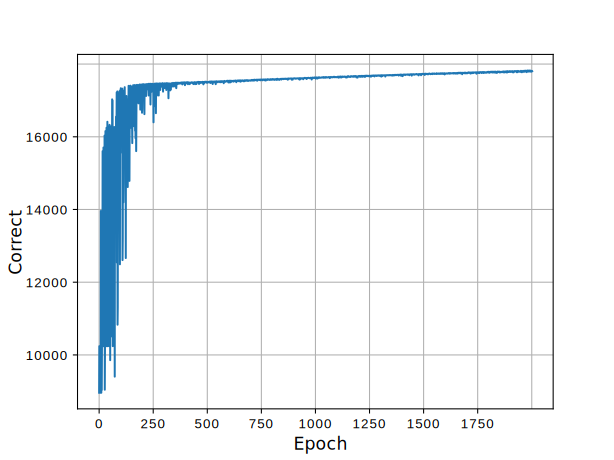
\includegraphics[width=1\hsize]{./figures/learning_curvesinsqr128_32i_l_hilsinsqr128_32i_l2_hil_num_neuron64_ramdomselected_timesequence_epoch2000_batchsize128_mask10_eta30_transition0_loopnum9_r} 
\caption{Correct number of the classification (64~output electrodes, including errors caused by switching of the input signals).}
\label{fig:nc64}
\end{figure}

64個の電極を使用した時の結果が図\ref{fig:result64}である。正弦波を入力している時間帯は0、矩形波を入力している時間帯は1に近い出力が得られており、適切に分類できていることがわかる。入力信号が切り替わる部分で中間的な出力が出ているのは、リザバーが時系列データを扱っていることを表している。またこのときの、エポック数に対する目標出力と実際の出力のRMSEを示したものが\ref{fig:lc64}、検証データの正解数を示したものが図\ref{fig:nc64}であり、学習がうまく進んでいることがわかる。なお、正解数は出力が0.5未満のときは0(正弦波)、0.5以上のときは1(矩形波)と判定されたものとした。

\begin{figure}
\centering
%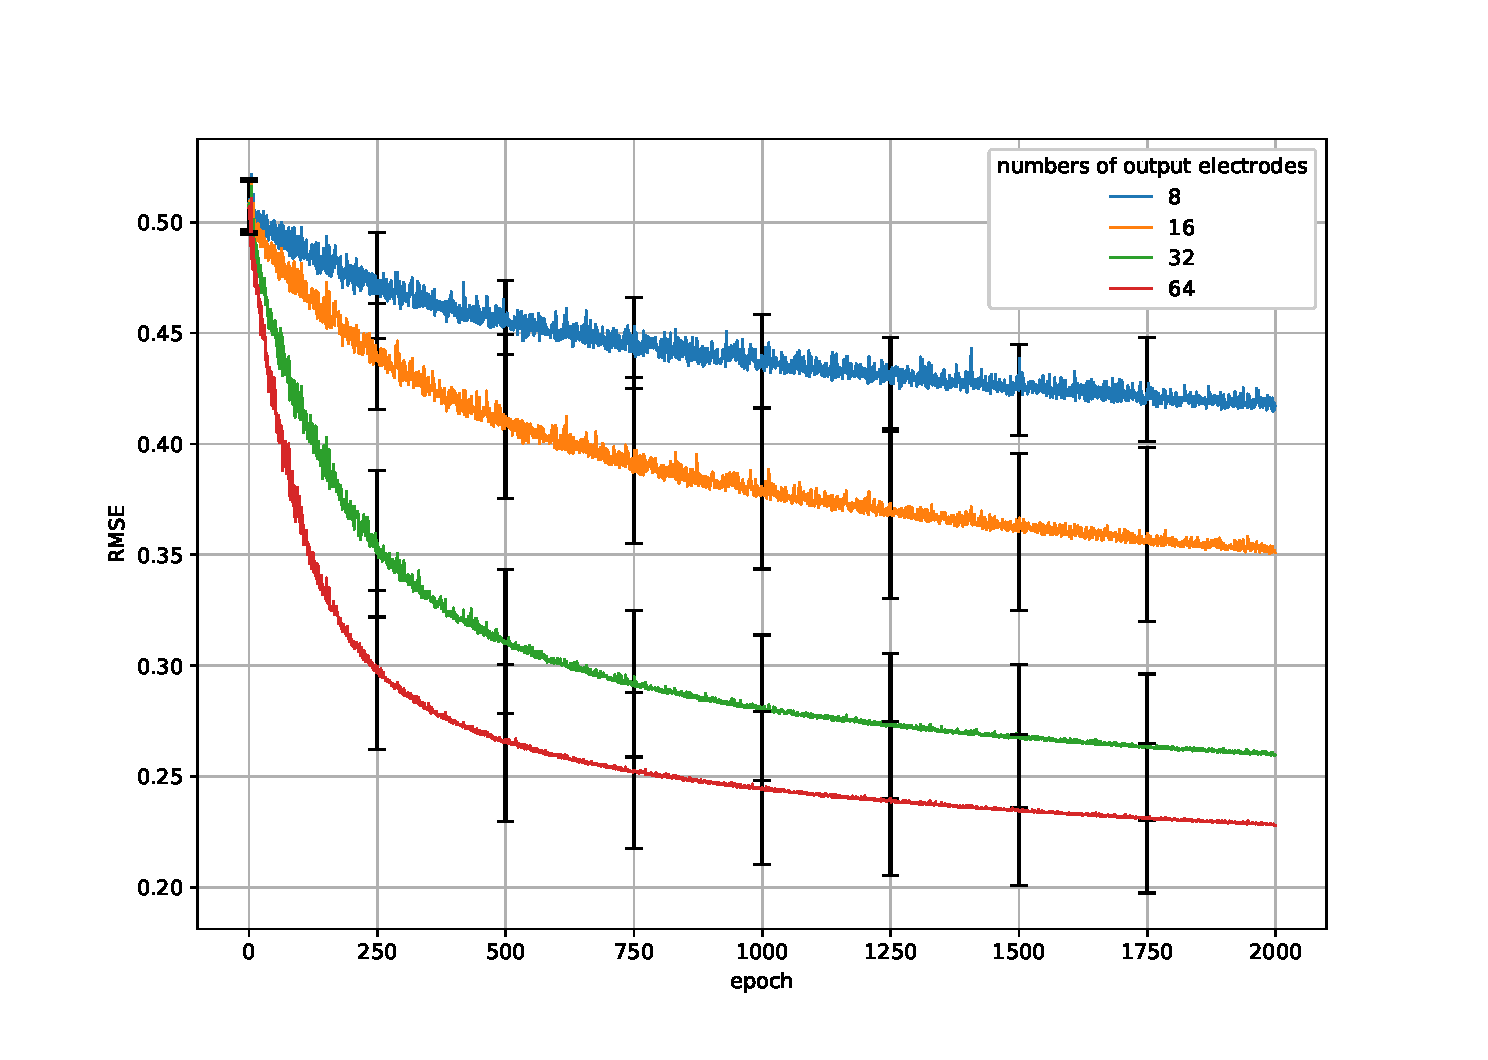
\includegraphics[width=1\hsize]{./figures/loop_rmse.eps} 
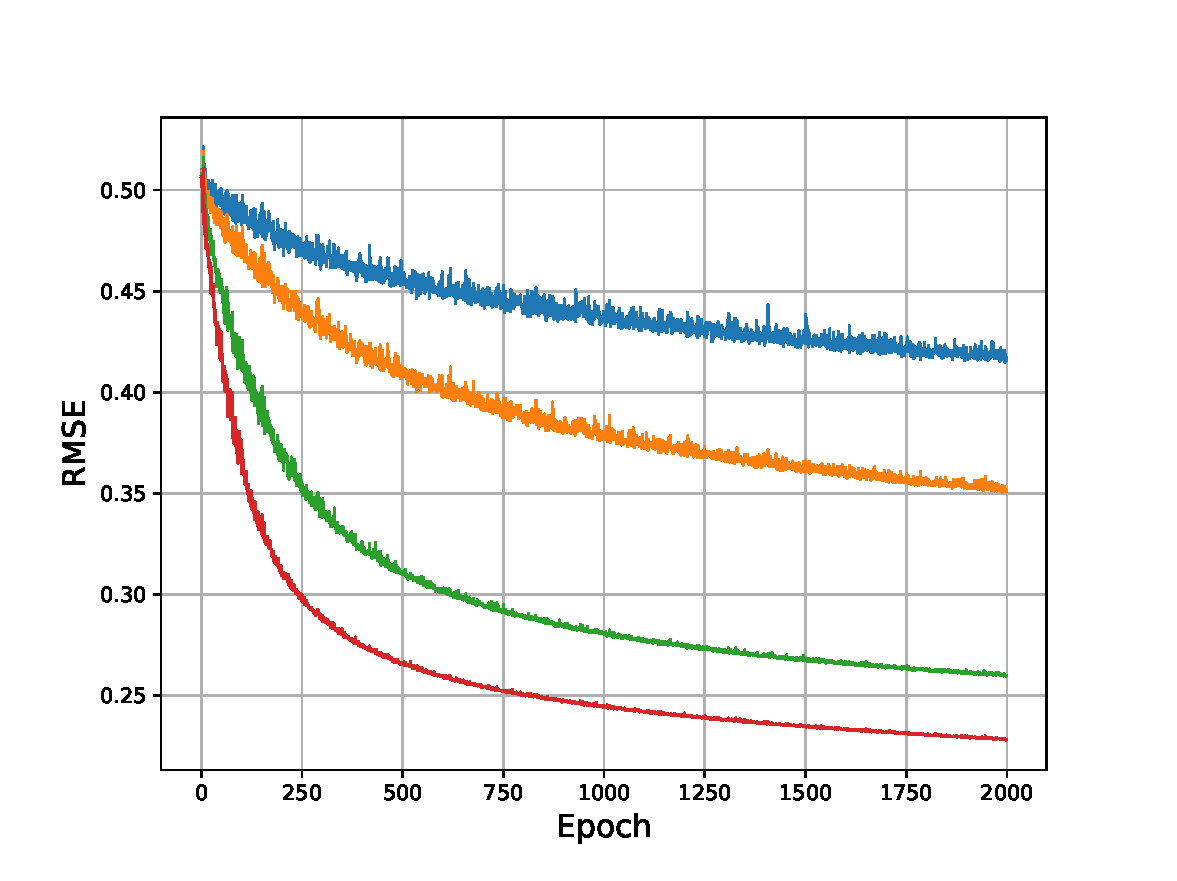
\includegraphics[width=1\hsize]{./figures/rmsevs_r2} 
\caption{RMSE when the number of output electrodes are changed.}
\label{fig:rmsevs}
\end{figure}

8、16、32、64個のランダムに選択した電極を利用して学習を行った場合の、出力と教師信号のRMSEを示したのが図\ref{fig:rmsevs}である。ランダムに選択した場合のRMSEや正解数はばらつきが大きいためそれぞれ10回づつ学習を行い、それらの分散をエラーバーに示した。図\ref{fig:rmsevs}から電極数が多いほど学習が早くなっていることがわかる。これは図\ref{fig:weightsinsqr128_32i}における有用情報が得られる場所に電極が配置される確率が高まるからだと考えられる。実行するタスクがある程度決まったものであれば、図\ref{fig:weightsinsqr128_32i}を利用して有用情報が多く得られる場所に出力電極を配置することで、性能が高いデバイスを作成できる可能性がある。ただしその場合、未知の入力への汎化能力が低下すると考えられるので、配置場所にはある程度のランダム性はあったほうが望ましいと考えられる。

\section{結論と今後の方針}
\label{sec:conclusion}
今回、まず正弦波矩形波の波形分類タスクについてスピン波の伝搬や振幅の分布を観察し、リザバーコンピューティングに必要とされるような複雑な応答が得られたことを確認した。
次に、仮想的に全メッシュにくまなく出力電極を配置し学習を行い、荷重分布から得られる有用情報分布を確認することで、理想的な出力電極の大きさが数十~nmであることを確認した。
そして、現実的に64個の出力電極という実装可能な構成を持ったスピン波リザバーが、波形分類タスクを行うことができることをシミュレーション解析上で示した。また8個、16個、32個の出力電極でも同様の分類の学習を行い、この個数の範囲では出力電極は多ければ多いほど良い、ということがわかった。
以上の結果は、現実的な構成のスピン波リザバーが実用的タスクを行えるということを示し、また物理的実装をする際の出力電極の大きさ、個数を決める指針となる。


\bibliographystyle{IEEEtran}
\bibliography{C:/Users/sprol/bib/mybib_reservoir,C:/Users/sprol/bib/cvnn_bib_utf,C:/Users/sprol/bib/mybib_InSAR,C:/Users/sprol/bib/mybib_landmine,C:/Users/sprol/bib/mybib_coherent_opt,mybiblio,mybiblio}

\addcontentsline{toc}{section}{発表文献}
\section*{発表文献}
{\bf 論文誌論文}
\begin{enumerate}
\item Takehiro Ichimura, Ryosho Nakane, Gohei Tanaka, Akira Hirose. "Waveform classification using spin-wave-based phisical reservoir computing", IEEE Transactions on Neural Network and Learning System, in preparation.
\end{enumerate}


{\bf 国内研究会発表}
\begin{enumerate}
\item 市村剛大、中根了昌、田中剛平、廣瀬明、「スピン波リザバーコンピューティングにおける有用情報の空間分布」、ニューロコンピューティング研究会(NC)、東京、2019年3月
\item 市村剛大、中根了昌、田中剛平、廣瀬明、「スピン波を用いたリザバーコンピューティングデバイスにおける荷重の空間分布」、CS-2-8、電子情報通信学会総合大会、東京、2019年3月
\item 市村剛大、中根了昌、田中剛平、廣瀬明、「スピン波リザバーコンピューティングチップにおける実空間情報分布」、P1-30、日本神経回路学会全国大会(JNNS)、東京、2019年9月
\end{enumerate}

\end{document}
%%%%%%%%%%%%%%%%%%%%%%%%%%%%%%%%%%%%%%%%%%%%%%%%%%%%%%%%%%%%%%%%%%%%%%%%%%%%%%%%%%%%%%%%%%%%%%%%%%%%%%%%%%%%%%%%%%%%%%%%%%%%%%%%%%%%%%%%%%%%%%%%%%%%%
%trash

\begin{eqnarray}
\label{eq:lsm1}
	\tau\dot{x}(t) = -x(t) + f_{NL}[x(t-\tau_{D})],
\end{eqnarray}
